\section{Grundlegende Datenstrukturen und deren Algorithmen}
Algorithmen manipulieren dynamische Mengen von Elementen (Einabe
$\rightarrow$ Ausgabe). Diese Mengen werden durch verschiedene
abstrakte Datenstrukturen realisiert. Diese Datenstrukturen
unterscheiden sich insbesondere durch Effizienz in Bezug auf
Manipulationen (Einfügen, Löschen etc.). Die Wahl der richtigen
Datenstruktur hängt also davon ab, welche Operationen der
zugrundeliegende Algorithmus verwendet und wie effizient die
Datenstruktur diese Operationen umsetzt. Im Folgenden sollen einige
grundlegenden Datenstrukturen eingeführt und deren Vor- und Nachteile
diskutiert werden.

Die Dantestrukturen sollten also insbesondere nicht für genau einen
Algorithmus entworfen werden, sondern wiederverwendbar gestaltet sein
und von unnötigen Details abstrahieren. Darüberhinaus sollten sie
unabhängig ihrer späteren Implementierung in einer konkreten
Programmiersprache spezifiziert werden.

Wir wollen nun zunächst Graphen und Bäume eingeführen, welche die
Grundlage für viele der nachfolgend eingeführten Datenstrukturen
bilden.

\subsection{Graph}
\begin{defi}
	Ein Graph $G$ ist ein geordnetes Paar $(V,W)$, wobei $V$ eine Menge von Knoten und $E$ eine Menge von Kanten bezeichnet. Dabei sind Kanten paarweise Verbindungen zwischen Knoten. Diese Kanten können mit sog. Gewichten versehen werden. Grundsätzlich unterscheidet man \emph{gerichtete} und \emph{ungerichtete} Kanten. Sind alle Paare $(v_1, v_2) \in E$ gerichtet, d. h. $(v_1, v_2) \neq (v_2, v_1)$, dann spricht man von einem gerichteten Graphen (\emph{Digraph}). Ein ungerichteter Graph, bei dem jeder Knoten mit allen anderen Knoten verbunden ist, heißt \emph{vollständig}.
\end{defi}

\begin{bsp}
	Abbildung \ref{digraph} zeigt ein Beispiel für einen Digraphen mit $V=\{1,2,3,4,5,6\}$ und den Kanten
	\begin{gather*}
		E=\{(1,4), (2,1), (2,3), (3,6), (4,2), (4,3), (4,5), (5,1), (5,3), (5,6), (6,4)\}.
	\end{gather*}
	\label{bsp:digraph}
\end{bsp}

\begin{figure}[!h]
	\centering
	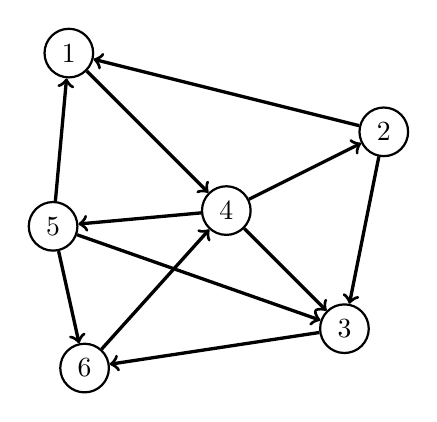
\begin{tikzpicture}
		\begin{scope}[every node/.style={circle,thick,draw}]
			\node (A) at (0,0) {1};
			\node (B) at (4,-1) {2};
			\node (C) at (3.5,-3.5) {3};
			\node (D) at (2,-2) {4};
			\node (E) at (-0.2,-2.2) {5};
			\node (F) at (0.2,-4) {6};
		\end{scope}

		\begin{scope}[every edge/.style={draw=black, very thick}]
			\path [->] (A) edge (D);
			\path [->] (B) edge (A);
			\path [->] (B) edge (C);
			\path [->] (C) edge (F);
			\path [->] (D) edge (B);
			\path [->] (D) edge (E);
			\path [->] (D) edge (C);
			\path [->] (E) edge (A);
			\path [->] (E) edge (F);
			\path [->] (E) edge (C);
			\path [->] (F) edge (D);
		\end{scope}
	\end{tikzpicture}
	\caption{Beispiel für einen Digraphen}
	\label{digraph}
\end{figure}

\begin{proposition}
	Sei $G=(E, V)$ ein Graph. Dann gilt:
	\begin{enumerate}[label=(\roman*)]
		\item Für die Anzahl von Kanten in einem Digraphen ohne Schleifen und Mehrfachkanten gilt
		      \begin{gather*}
			      |E| \le |V|(|V| - 1).
		      \end{gather*}

		\item Für die Anzahl von Kanten in einem ungerichteten Graphen ohne Schleifen und Mehrfachkanten gilt
		      \begin{gather*}
			      |E| \le \frac{1}{2} |V|(|V| - 1).
		      \end{gather*}
	\end{enumerate}
	In vollständigen Graphen gilt jeweils Gleichheit.
\end{proposition}

\begin{proof}[Beweis (nur für $(i)$ )]
	Jeder Knoten hat höchstens alle Knoten außer sich selbst als Nachbar, er hat also $|V| - 1$ Nachbarn. Da dies für jeden Knoten des Graphen möglich ist folgt die Behauptung.
\end{proof}

Eine weitere Möglichkeit Graphen anzugeben sind sog. \emph{Adjazenzlisten} oder \emph{Adjazenzmatrizen}. Hierbei listet man für die jeweiligen Knoten alle Nachbarn auf (Adjazenzliste) bzw. setzt in einer Matrix den Eintrag $a_{ij}$ auf $1$, falls es eine Kante vom Knoten $v_1$ nach $v_2$ gibt, bzw. allgemein:
\begin{defi}[Adjazenzmatrix]
	Eine Adjazenzmatrix eines Graphen $G=(V,E)$ ist eine $|V| \times |V|$-Matrix $A = (a_{ij})$ mit
	\begin{gather*}
		a_{ij} = \begin{cases}
			1 & \text{falls } (i,j) \in E \\
			0 & \text{sonst.}
		\end{cases}
	\end{gather*}
\end{defi}

\begin{anm}
	Offensichtlich sind Adjazenzmatrizen von ungerichteten Graphen symmetrisch.
\end{anm}

Für den im Beispiel \ref{bsp:digraph} definierten Graph sieht die Adjazenzmatrix folgendermaßen aus:
\begin{gather*}
	\bordermatrix{
		& 1 & 2 & 3 & 4 & 5 & 6 \cr
		1 & 0 & 0 & 0 & 1 & 0 & 0 \cr
		2 & 1 & 0 & 1 & 0 & 0 & 0 \cr
		3 & 0 & 0 & 0 & 0 & 0 & 1 \cr
		4 & 0 & 1 & 1 & 0 & 1 & 0 \cr
		5 & 1 & 0 & 1 & 0 & 0 & 1 \cr
		6 & 0 & 0 & 0 & 1 & 0 & 0 \cr
	}
\end{gather*}

Für gewichtete Graphen eignet sich die Darstellung in Form von Adjazenzmatrizen auch: hierbei kann anstatt des Wertes $1$ in der Adjazenzmatrix einfach das Gewicht der jeweiligen Kante eingetragen werden.

Für gerichtete Graphen wollen wir nun weitere Begriffe einführen:

\begin{defi}
	Sei $G=(V,E)$ ein gerichteter Graph. Dann definieren wir
	\begin{itemize}
		\item die eingehende Nachbarmenge von $v \in V$:
		\begin{gather*}
			N^{+}(v) = \{u \in V \mid (u,v) \in E \}
		\end{gather*}

		\item die ausgehende Nachbarmenge von $v \in V$:
		\begin{gather*}
			N^{-}(v) = \{w \in V \mid (v,w) \in E \}
		\end{gather*}

		\item den Eingangsgrad von $v \in V$:
		\begin{gather*}
			deg_{in}(v) = \big| N^{+}(v) \big|
		\end{gather*}

		\item den Ausgangsgrad von $v \in V$:
		\begin{gather*}
			deg_{out}(v) = \big| N^{-}(v) \big|
		\end{gather*}
	\end{itemize}
\end{defi}

Setzt man Graphen als Datenstruktur ein, so ist es häufig das Ziel, den (kürzesten) Weg zwischen zwei Knoten zu finden. Dies führt uns zur nächsten

\begin{defi}[Pfade]
	Es sei $G=(V,E)$ ein Graph. Ein Pfad ist eine Folge von paarweise verschiedenen Knoten $u_1, \dots, u_k \in V$, wobei $(u_i, u_{i+1}) \in E$ für alle $i \in \{1, \dots, k-1\}$. \\

	Die Länge eines Pfades ist die Anzahl der Kanten (falls die Kanten von $G$ nicht gewichtet sind) bzw. die Summe der Kantengewichte. Dabei sei $d(u,v)$ die Länge des kürzesten Pfades von $u$ nach $v$. Der Durchmesser $D$ sei definiert durch $D = \underset{u,v \in V}{\max}{d(u,v)}$. \\

	Ist $v_1 = v_k$, so heißt der Pfad $(v_1, \dots, v_k)$ Zyklus \footnote{Hierbei wird allerding i. d. R. nicht verlangt, dass $(v_1, \dots, v_k)$ ein Pfad ist -- es genügt dass $(v_1, \dots, v_k)$ ein Weg ist (die Knoten müssen also nicht paarweise verschieden sein).}. Gilt zusätzlich $v_i \neq v_j$ für $i,j \in \{1, \dots, k-1\}$ mit $i \neq j$, dann heißt der Pfad Kreis.
\end{defi}

\begin{defi}
	Es sei $G = (V,E)$ ein Graph mit $|V| \ge 1$. $G$ heißt \emph{zusammenhängend}, falls für jedes Knotenpaar $(u,v)$ mit $u,v \in E$ ein Weg von $u$ nach $v$ in $G$ exisitert.
\end{defi}

\subsubsection{Breitensuche (Breadth-First-Search)}
Bei der Breitensuche handelt es sich um ein Verfahren zum Durchsuchen (oder nur Durchlaufen) der Knoten eines Graphen. Hierbei werden zunächst alle Knoten beschritten, die vom Ausgangsknoten direkt erreichbar sind. Erst danach werden Folgeknoten beschritten. Dazu verwendet man in der Regel eine Warteschlange (vgl. Abschnitt \emph{Queue}). \\ \\
Informell lässt sich die Breitensuche folgendermaßen beschreiben:
\begin{enumerate}
	\item Bestimme den Knoten, an dem die Suche beginnen soll, markiere ihn als besucht und füge ihn der Warteschlange hinzu
	\item Entnimm einen Knoten vom Beginn der Warteschlange
	\begin{itemize}
		\item Falls der entnommene Knoten der gesuchte Knoten ist, brich die Suche ab (und gebe den Knoten oder ``gefunden'' zurück)
		\item Andernfalls hänge alle unmarkierten Nachfolge diese Knoten ans Ende der Warteschlange an und markiere sie als besucht
	\end{itemize}
	\item Prüfe ob die Warteschlange leer ist. Falls ja, beende die Suche (gesuchtes Element wurde nicht gefunden)
	\item Wiederhole Schritt 2.
\end{enumerate}
Als Pseudocode könnte die Breitensuche folgendermaßen aussehen:
\begin{algorithm}[H]
	\caption{Breitensuche mit Startknoten $start$ und gesuchtem Knoten $goal$}
	 \begin{algorithmic}
		 \Procedure{bfs}{$start, goal$}
				\For{\textbf{all node} $i$} \Comment{Anfangs sind keine Knoten besucht}
					\State{$visited[i] \gets false$}
				\EndFor
				\State{$queue.$\Call{push}{$start$}}
				\State{$visited[start] \gets true$}

				\While{\textbf{not} $queue.$\Call{empty}{}}
					\State{$node \gets queue.$\Call{pop}{}}
					\If{$node$ \textbf{is} $goal$}
						\State{\Return{$true$}}
					\EndIf
					\For{$child$ \textbf{in} $neighbors[node]$}
						\If{\textbf{not} $visited[child]$}
							\State{$queue.$\Call{push}{$child$}}
							\State{$visited[child] \gets true$}
						\EndIf
					\EndFor
				\EndWhile
				\State{\Return{$false$}}
		 \EndProcedure
	 \end{algorithmic}
\end{algorithm}

\begin{proposition}[Laufzeit]
	Im schlechtesten Fall müssen alle möglichen Pfade zu allen möglichen Knoten betrachtet werden, daher gilt für die Laufzeit der Breitensuche
	\begin{itemize}
		\item Falls Adjazenzlisten benutzt werden: $\mathcal{O}(|V| + |E|)$
		\item Falls Adjazenzmatrizen benutzt werden: $\mathcal{O}(|V|^2)$.
	\end{itemize}
\end{proposition}

\begin{bsp}
	Interpretiert man einen Graphen als Baum und definiert die Reihenfolge der Nachfolger eines Knotens von links nach rechts, so würde man den Baum in Abbildung \ref{bfstree} Ebene für Ebene und innerhalb der Ebenen von links nach rechts durchlaufen und erhielte dann die Reihenfolge
	\begin{gather*}
		17 \rightarrow 4 \rightarrow 11 \rightarrow 18 \rightarrow 3 \rightarrow 9 \rightarrow 13 .
	\end{gather*}
\end{bsp}

\begin{figure}[!h]
	\centering
	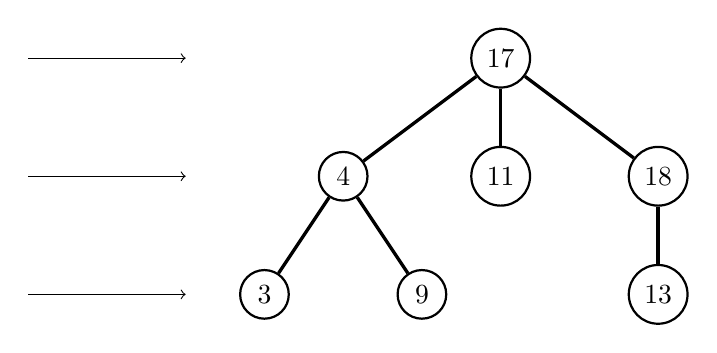
\begin{tikzpicture}
		\begin{scope}[every node/.style={circle,thick,draw}]
			\node (A) at (0,0) {17};
			\node (B) at (-2,-1.5) {4};
			\node (C) at (0,-1.5) {11};
			\node (D) at (2, -1.5) {18};
			\node (E) at (-3, -3) {3};
			\node (F) at (-1, -3) {9};
			\node (G) at (2, -3) {13};
		\end{scope}

		\begin{scope}[every edge/.style={draw=black, very thick}]
			\path [-] (A) edge (B);
			\path [-] (A) edge (C);
			\path [-] (A) edge (D);
			\path [-] (B) edge (E);
			\path [-] (B) edge (F);
			\path [-] (D) edge (G);
		\end{scope}

		\draw [->] (-6,0) -- (-4,0);
		\draw [->] (-6,-1.5) -- (-4,-1.5);
		\draw [->] (-6,-3) -- (-4,-3);


	\end{tikzpicture}
	\caption{Breitensuche in einem Baum}
	\label{bfstree}
\end{figure}
\subsubsection{Tiefensuche (Depth-First-Search)}
Wie auch die Breitensuche ist die \emph{Tiefensuche} ein Verfahren zum Suchen von Knoten in einem Graphen. Im Gegensatz zur Breitensuche wird ein Pfad zunächst vollständig in die Tiefe beschritten, bevor abzweigende Pfade beschritten werden.\\
Informell lässt sich die Tiefensuche folgendermaßen beschreiben:
\begin{enumerate}
	\item Bestimme den Startknoten
	\item Bestimme alle Nachfolger bzw. Nachbarn des Knotens und speichere alle noch nicht erschlossenen Nachfolger in einem Stack
	\item Rufe rekursiv für jeden Knotne in dem Stack die Tiefensuche auf
	\begin{itemize}
		\item Falls das gesuchte Element gefunden wurde breche ab
		\item Falls es keine nicht erschlossenen Nachfolger mehr gibt, lösche den obersten Knoten aus dem Stack und rufe für den jetzt oberen Knoten im Stack die Tiefensuche auf
	\end{itemize}
\end{enumerate}

In Pseudocode könnte die Tiefensuche folgendermaßen aussehen:
\begin{algorithm}[H]
	\caption{Tiefensuche mit Startknoten $start$ und gesuchtem Knoten $goal$}
	\begin{algorithmic}
		\Procedure{dfs}{$start, goal$}
			\If{$start$ \textbf{is} $goal$}
				\State{\Return $start$}
			\EndIf
			\State{$stack \gets$ \Call{neighbors}{$start$}}
			\While{$stack$ \textbf{is not empty}}
				\State{$node \gets$ \Call{pop}{$stack$}}
				\State{\Call{dfs}{$node, goal$}}
			\EndWhile
		\EndProcedure
	\end{algorithmic}
\end{algorithm}

\begin{bsp}
	Mit dem selben Baum wie in Abbildung \ref{bfstree} erhält man nun mit der Tiefensuche (siehe Abb. \ref{dfstree}) die Reihenfolge
	\begin{gather*}
		17 \rightarrow 4 \rightarrow 3 \rightarrow 9 \rightarrow 11 \rightarrow 18 \rightarrow 13 
	\end{gather*}
\end{bsp}

\begin{figure}[!h]
	\centering
	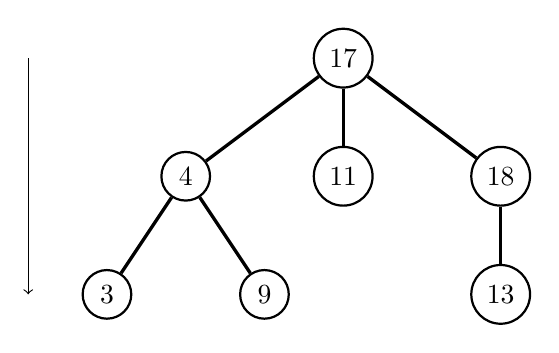
\begin{tikzpicture}
		\begin{scope}[every node/.style={circle,thick,draw}]
			\node (A) at (0,0) {17};
			\node (B) at (-2,-1.5) {4};
			\node (C) at (0,-1.5) {11};
			\node (D) at (2, -1.5) {18};
			\node (E) at (-3, -3) {3};
			\node (F) at (-1, -3) {9};
			\node (G) at (2, -3) {13};
		\end{scope}

		\begin{scope}[every edge/.style={draw=black, very thick}]
			\path [-] (A) edge (B);
			\path [-] (A) edge (C);
			\path [-] (A) edge (D);
			\path [-] (B) edge (E);
			\path [-] (B) edge (F);
			\path [-] (D) edge (G);
		\end{scope}

		\draw [->] (-4,0) -- (-4,-3);


	\end{tikzpicture}
	\caption{Tiefensuche in einem Baum}
	\label{dfstree}
\end{figure}

\subsection{Bäume}
Ein Baum ist ein spezieller Typ von Graph, der zusammenhängend ist und
keine geschlossenen Pfade (Kreise) enthält. Die Knoten mit Grad 1
heißen Blätter (sie haben insbesondere Ausgangsgrad 0). Beispiele für
Bäume haben wir bereits in Abbildung \ref{bfstree} und \ref{dfstree}
gesehen. In der Regel betrachten wir nur gerichtete Bäume, die einen
ausgezeichneten Startknoten besitzen, die sog. Wurzel. Die Wurzel
zeichnet sich dadurch aus, dass sie der einzige Knoten mit
Eingangsgrad 0 ist.

Man erkennt leicht, dass es zwischen zwei Knoten eines Baums nur genau
einen Pfad geben kann. Außerdem gilt für die Anzahl der Kanten eines
Baums $G = (E,V)$:
\begin{gather*}
  |E| = |V| - 1,
\end{gather*}
da es zu jedem Knoten eine Kante gibt, außer zur Wurzel.\\

Im Folgenden betrachten wir hauptsächlich \emph{Binärnäume}, welche
sich dadurch auszeichnen, dass jeder Knoten eines Binärbaums nur
höchstens zwei direkte Nachkommen (\emph{Kinder}) haben kann.  Als
\emph{Tiefe} eines Knotens bezeichnen wir die Anzahl der Kanten bis
zur Wurzel. Dabei ist die Höhe des Baumes die maximal auftretende
Tiefe.\footnote{Oft definiert man jedoch die Höhe des leerens Baums
  als $0$, muss also zur Anzahl der Kanten noch $1$ addieren.} Haben
alle Blätter die gleiche Tiefe, so heißt der Baum vollständig.

\subsubsection{Suche in Bäumen}
Wir unterscheiden zunächst die folgenden drei Varianten, um einen Baum
zu durchlaufen:
\begin{defi}
  Es sei $T$ ein geordneter Baum mit Wurzel $r$ und Teilbäumen
  $T_1, \dots, T_m$.
  \begin{enumerate}
  \item[(a)] Wenn $T$ in \emph{Postorder} durchlaufen wird, dann
    werden (rekursiv) die Teilbäume $T_1, \dots, T_m$ nacheinander
    durchlaufen und danach wird die Wurzel $r$ besucht.
  \item[(b)] Wenn $T$ in \emph{Präorder} durchlaufen wird, dann wird
    zuerst $r$ besucht und dann werden die Teilbäume $T_1, \dots, T_m$
    (rekursiv) durchlaufen.
  \item[(c)] Wenn $T$ in \emph{Inorder} durchlaufen wird, wird zuerst
    $T_1$ (rekursiv) durchlaufen, sodann wird die Wurzel $r$ besucht
    und letzlich werden die Teilbäume $T_2, \dots, T_m$ (rekursiv)
    durchlaufen.
  \end{enumerate}
\end{defi}

\subsubsection{Binärer Suchbaum}
Ein \emph{binärer Suchbaum} ist ein binärer Baum, bei dem den Knoten
Schlüssel zugewiesen werden und die Schlüssel des linken Teilbaums
eines Knotens nur kleiner (oder gleich) und die des rechten nur größer
(oder gleich) als der Schlüssel des Knotens selbst sind. Sie lösen
(wie auch andere Suchbäume) das
sog. \emph{Wörterbuchproblem}. Angenommen ist eine große Anzahl von
Schlüsseln, denen jeweils ein Wert beigegeben ist. In einem Wörterbuch
deutsch–englisch ist das deutsche Wort der Schlüssel und englische
Wörter sind der gesuchte Wert. Ähnlich verhält es sich bei einem
Telefonbuch mit Namen und Adresse als Schlüssel und der Telefonnummer
als dem gesuchten Wert.

In beiden Beispielen sind die Schlüssel üblicherweise sortiert, was es
ermöglicht das Suchen nach Schlüsseln deutlich zu beschleunigen: Man
schlägt das Buch zunächst in der Mitta auf und überprüft, ob der
Schlüssel gefunden wurde. Falls er nicht gefunden wurde, der gesuchte
Schlüssel aber kleiner ist, als der betrachtete, kann man nun die
hintere Hälfte des Buches schon ausschließen. So kann man nun rekursiv
mit der entsprechenden anderen Hälfte fortfahren und gelangt so bei
$n$ Schlüsseln mit maximal $\lceil \log_2(n+1) \rceil $ Vergleichen
zum Ziel.\footnote{Dieses Verfahren nennt man \emph{Binäre Suche}}

Einen Binärbaum würde man so aufbauen, dass zuerst ein Element als
Wurzel eingefügt wird. Wird ein neues Element eingefügt, dessen
Schlüssel kleiner ist als der der Wurzel, wird es in den linken
Teilbaum eingefügt (rekursiv mit dem linken Kind als neue Wurzel,
solange bis man es als Blatt einfügen kann). Analog verfährt man für
Elemente mit größerem Schlüssel.

Hierbei kann es natürlich vorkommen, dass der Baum nicht balanciert
ist oder im Extremfall sogar zur lineare Liste wird (wenn man immer
nur größere bzw. immer nur kleinere Elemente einfügt). Aus dieser
Problematik heraus sind einige Varianten des Binären Suchbaums
entstanden, die die Baumstruktur beim Einfügen oder Löschen so
verändern, dass der Baum balanciert wird oder die Struktur zumindest
praktischer wird.

\subsection{Hashing und Hashtabellen}
Hashtabellen sind eine weitere Datenstruktur, die wie jede andere
Datenstruktur (Arrays, Heaps, Bäume) auch Stärken und Schwächen
hat. Hashtabellen eignen sich besonders, so lange wir nur eine Menge
von Daten benötigen, in die wir schnell einfügen, löschen und in der
wir suchen können, sind Hashtabellen meist sehr
effizient.\footnote{Dabei hängt die Effizienz der Hashtabelle
  maßgeblich von der Qualität der verwendeten Hashfunktion ab, die für
  die Art der verwendeten Daten geeignet sein muss.}

Die zugrundeliegende Idee ist es, aus den zu speichernden Elementen
selbst deren Position in einer Tabelle zu schließen. Dann müsste man
beim Suchen einen Elements nur dessen Position berechnen und könnte
direkt an die richige Stelle in der Tabelle springen.

\begin{defi}
  Eine \emph{Hashtabelle} ist eine Datenstruktur, welche mit Hilfe
  einer Funktion $h : U \rightarrow D$ -- die sog. \emph{Hashfunktion}
  -- die Position berechnet, an der der Schlüssel $u \in U$ im
  Elementebereich (also in der Hashtabelle) $D \subset \mathbb{N}$
  gespeichert werden soll. Der Elementbereich $D$ ist dabei eine
  natürliche Zahl in $\{0, 1, \dots, m-1\}$, wobei $m$ die Länge der
  Hashtabelle ist.
\end{defi}

Die Hashfunktion berechnet also für ein gegebenes Element dessen
Position in einer Tabelle. Sucht man nun ein Element, oder will ein
neues Element einfügen, kann man mit Hilfe der Hashfunktion die
Position des Elements berechnen und kann dann in konstanter Zeit
($\mathcal{O}(1)$) direkt an die entsprechende Stelle in der Tabelle
springen.
Hashtabellen sind also insbesondere nur geeignet, wenn aus den zu speichernden Elementen einfach eindeutige Schlüssel generiert werden können. \\
Gute Hashfunktion sollten
\begin{itemize}
\item surjektiv sein, d.h. die ganze Tabelle ausnutzen
\item die Schlüssel möglichst gleichmäßig verteilen
\end{itemize}

\begin{anm}
  In der Regel gilt $|U| > |D|$, es gibt also mehr Schlüssel als
  Plätze in der Hashtabelle.\footnote{Die Schlüsselmenge zu
    verkleinern ist ja gerade einer der Gründe, Hashtabellen zu
    benutzen.} Da die Hashfunktion i. A. auch nicht injektiv ist, kann
  es sein, dass verschiedene Elemente (bzw. verschiedene Schlüssel)
  auf denselben Index (Hashwert) abgebildet werden. Dies bezeichnet
  man als \textbf{Kollision}. Es müssen also Strategien gefunden
  werden, die solche Kollisionen erkennen und behandeln.
\end{anm}

\subsubsection{Hashverfahren mit Verkettung}
Wir wollen in den Folgenden Abschnitten einige Möglichkeiten
diskutieren, Kollisionen zu behandeln. Eine intuitive Möglichkeit ist
es, bei einer Kollision einfach mehrere Elemente an der selben Stelle
in der Hashtabelle zu speichern, indem man für jeden Eintrag der
Hashtabelle eine Liste speichert, der man dann die kollidierenden
Elemente hinzufügt.

\subsubsection{Hashtabelle mit Sondierung}
\Large ToDo \normalsize

\subsection{Heap}
Ein \emph{Heap} (deutsch: Haufen) ist eine auf Bäumen basierende
Datenstruktur.


%%% Local Variables:
%%% mode: latex
%%% TeX-master: "../main"
%%% End:
